\section{Scene}

Scena sadrži sve objekte igre koji se koriste. Scena nam može služiti za kreiranje izbornika, ukoliko igra ima više levela, svaki level će se nalaziti u svojoj sceni. Preko scene uređujemo okolinu, postavljamo objekte i prepreke. Kada selektiramo neki objekt u sceni pojavit će se strelice preko kojih možemo objekt pomicati prema x, y i z osi, možemo povećavati, smanjivati ili rotirati objekt ovisno o selektiranoj opciji na alatnoj traci. Scena zapravo sve sklopljene elemente pretvara u jedan sadržaj. 



\subsection{Main menu}
Ovo je početna scena u igri. Scena sadrži platno sa tekstom i dva botuna te objekt "plane" na kojega je zaljepljena slika radi boljeg ugođaja. Klasa koja upravlja sa ovom scenom smještena je u "Main Camera" objektu. Pritiskom na jedan od botuna pozove se događaj "On Click()".

\begin{center}
	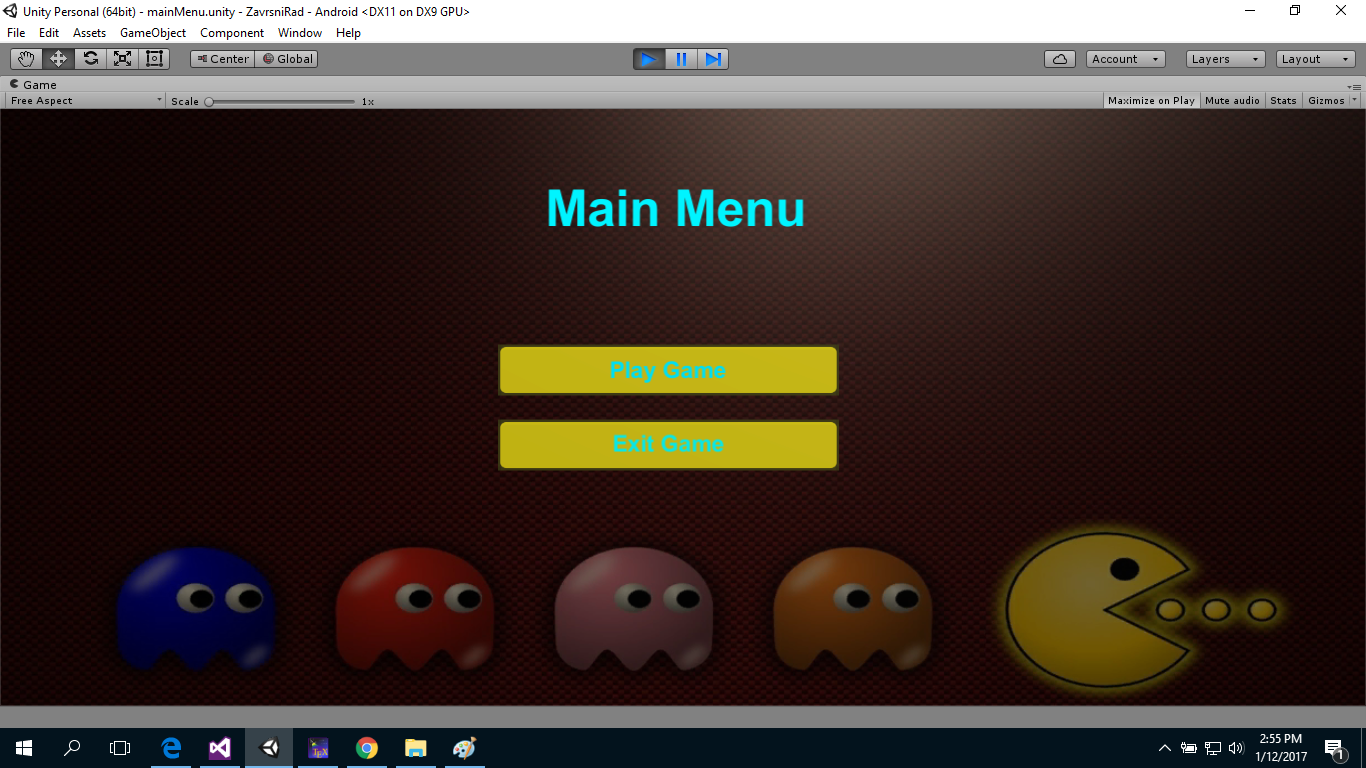
\includegraphics[scale=0.35]{scena1.png}
	
	Slika 3: Scena "Main Menu"
\end{center}

\newpage
\subsection{Game}
"Game" je glavna scena na koju korisnik dolazi pritiskom botuna "Play" na "Main Menu" sceni. Sadrži sve dolje napisane objekte i njihove komponente. Također sadrži i platno koje se pojavljuje po potrebi i preko kojeg se može vratiti na početnu scenu. Platno na "Game" sceni i platno na "Main menu" sceni imaju istu skriptu "Main Menu" s kojom se navigira između ove dvije scene. Svaka scena koristi svoje funkcije. "Main Menu" scena ima mogučnost izlaska iz igre i prelazak na scenu "Game", a scena "Game" ima  mogučnost prelaska na scenu "Main Menu" i ponovno igranje igre. Platno u "Game" sceni se pojavljuje ukoliko jedan od objekata "Ghost" se sudari sa glavnim objektom "Player" ili ako istekne određeno vrijeme predviđeno za prelazak igre. Objekti "Ghost" i "Player" su napravljeni u blender alatu dok su svi ostali objekti u ovoj sceni napravljeni u unity-u. Na ove objekte su zaljepljene slike radi boljeg ugođaja tokom igranja igre.


\begin{center}
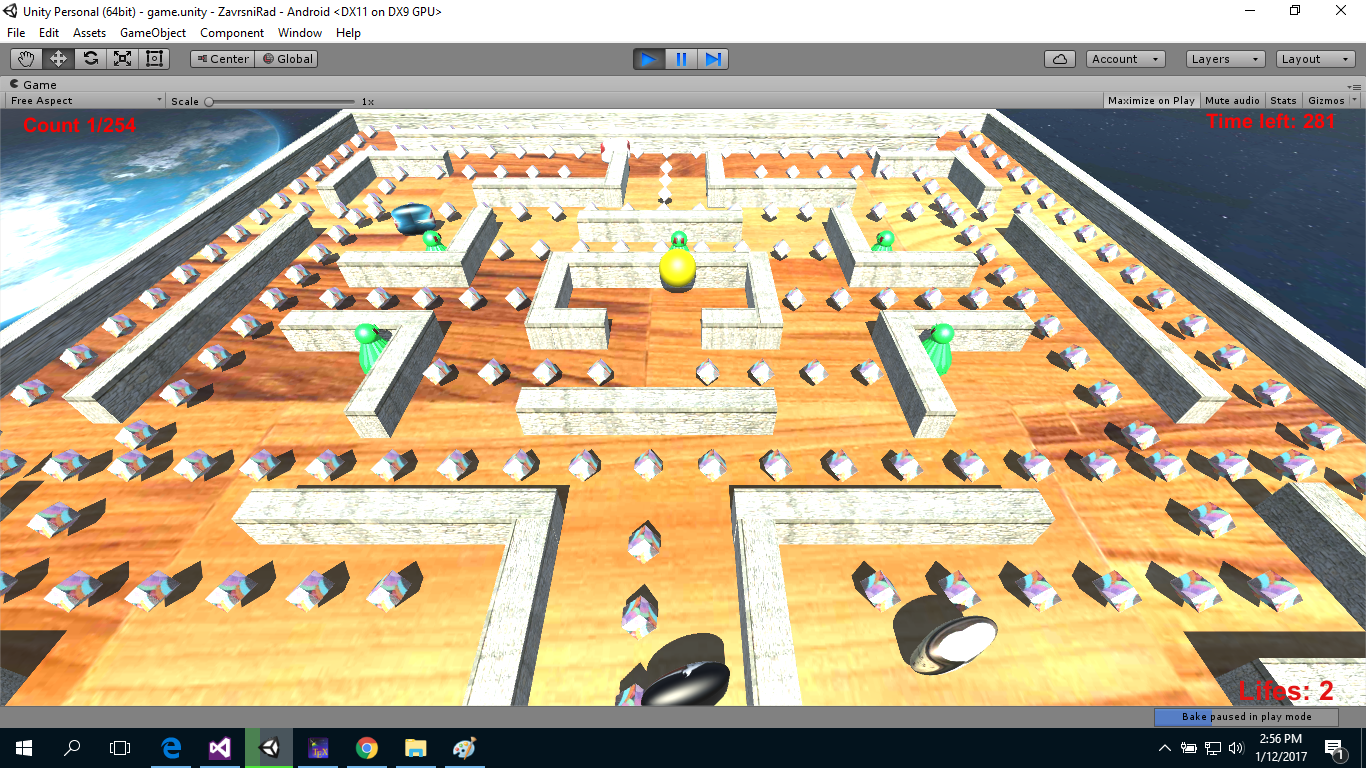
\includegraphics[scale=0.35]{scena2.png}

Slika 4: Scena "Game"
\end{center}
